\section{Auswertung}
\label{sec:Auswertung}


\begin{table}
  \centering
  \caption{Maße des runden und des eckigen Stabes}
  \sisetup{table-format=3.2}
  \begin{tabular}{l
      S
      S
      }
    \toprule
    & \multicolumn{1}{c}{Runder Stab} & \multicolumn{1}{c}{Eckiger Stab} \\
    \midrule
    {$l\mathbin{/}\si{mm}$} & 592,0 &602,0\\
    {$l_{\text{Lit}}\mathbin{/}\si{mm}$} & 551,82 & 591,18\\
    {$d$\,bzw.\,$h\mathbin{/}\si{mm}$}& 10,0 & 10,0 \\
    {$m\mathbin{/}\si{g}$}& 129,4 & 167,2 \\
    {$m_{\text{Lit}}\mathbin{/}\si{g}$}&120,9 & 164,0\\
    \bottomrule
  \end{tabular}
\end{table}

Aus den bestimmten Daten der Stäbe wird die Dichte des Materials nach der Formel:
\begin{equation}
  \rho=\frac{m}{V}
\end{equation} mit $V$ = Volumen des Stabs, zu
$\rho_{\text{r}} = \qty{2783,06}{\kilo\gram\per\cubic\meter}$, sowie  $\rho_{\text{e}}=\qty{2777,41}{\kilo\gram\per\cubic\meter}$ bestimmt.
Aus dem Vergleich mit Literaturwerten \cite{Dichte} wird klar, dass es sich um Aluminium handelt.

Außerdem wird das Flächenträgheitsmoment $I_{\text{r}}$  der Stäbe bestimmt. Bei einem runden Querschnitt wird dafür die Formel \cite{flaeche}
\begin{equation}
  I_{\text{r}} = \frac{\pi (d/2)^4}{4}.
\end{equation} verwendet.
Das Flächenträgheitsmoment für den runden Stab beträgt also: 
\begin{equation*}
  I_{\text{r}} = \qty{4,91e-10}{\meter\tothe{4}}.
\end{equation*}

Das Flächenträgheitsmoment des eckigen Stabes mit quadratischem Querschnitt berechnet sich nach der Formel \cite{flaeche}:
\begin{equation}
  I_{\text{e}} = \frac{b^4}{12}.
\end{equation}
Das Flächenträgheitsmoment für den eckigen Stab beträgt also: 
\begin{equation*}
  I_{\text{e}} = \qty{8,33e-10}{\meter\tothe{4}}.
\end{equation*}.

\pagebreak

\subsection{runder Stab, einseitige Einspannung}

\begin{table}[htbp]
  \centering
  \caption{Messung der Biegung des runden Stabs bei einseitiger Einspannung}
  \label{tab:runds}
  \sisetup{table-format=2.1}
  \begin{tabular}{S[table-format=3.0] S[table-format=1.2]}
    \toprule
    {$x \mathbin{/} \si{\milli\meter}$} & {$D(x) \mathbin{/} \si{\milli\meter}$}\\
    \midrule
    100 & 0,28\\
    125 & 0,35\\
    150 & 0,36\\
    175 & 0,45\\
    200 & 0,51\\
    225 & 0,62\\
    250 & 0,78\\
    275 & 0,93\\
    300 & 1,16\\
    325 & 1,34\\
    350 & 1,58\\
    370 & 1,78\\
    400 & 2,07\\
    425 & 2,30\\
    450 & 2,58\\
    475 & 2,79\\
    500 & 3,10\\
    525 & 3,48\\
    \bottomrule
  \end{tabular}
\end{table}


\begin{figure}
  \centering
  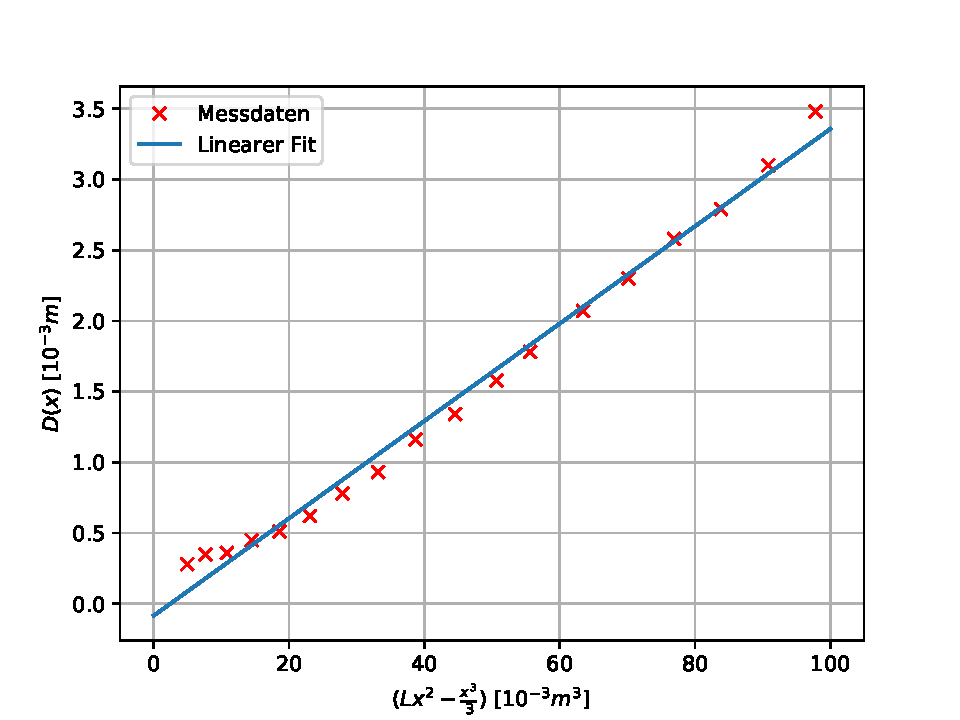
\includegraphics{content/plots/runde.pdf}
  \caption{Lineare Regression: runder Stab, einseitige Einspannung}
  \label{fig:LinRegrunde}
\end{figure}

a = 0.03440932788036839 ± 0.0008601488905380944
b = -0.08437719900299626 ± 0.04624542285827333

\pagebreak

\subsection{runder Stab, beidseitige Auflage}
test
\begin{table}
  \centering
  \caption{Messung der Biegung des runden Stabs bei beidseitiger Auflage}
  \label{tab:rundb}
  \sisetup{table-format=2.1}
  \begin{tabular}{S[table-format=3.0] S[table-format=1.2]}
    \toprule
    {$x \mathbin{/} \si{\milli\meter}$} & {$D(x) \mathbin{/} \si{\milli\meter}$}\\
    \midrule
    100 & 0,22\\
    125 & 0,25\\
    150 & 0,31\\
    175 & 0,30\\
    200 & 0,42\\
    225 & 0,38\\
    250 & 0,40\\
    275 \\
    300 & 0,40\\
    325 & 0,37\\
    350 & 0,41\\
    375 & 0,30\\
    400 & 0,31\\
    425 & 0,25\\
    450 & 0,21\\
    475 & 0,17\\
    500 & 0,12\\
    \bottomrule
  \end{tabular}
\end{table}

\begin{figure}
  \centering
  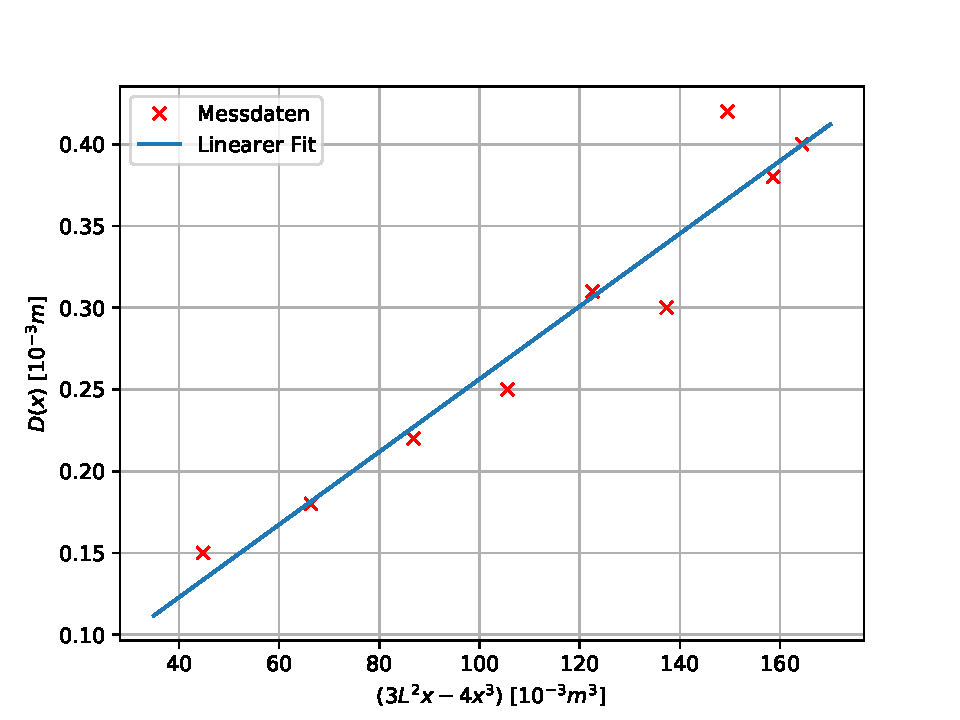
\includegraphics{content/plots/rundb1.pdf}
  \caption{Lineare Regression: runder Stab, beidseitige Auflage, $0<x<L/2$}
  \label{fig:LinRegrundb1}
\end{figure}

rundb1:
a = 0.0024963660231759333 ± 0.000427138613034415
b = -0.004118075387476106 ± 0.05756132336959278

\begin{figure}
  \centering
  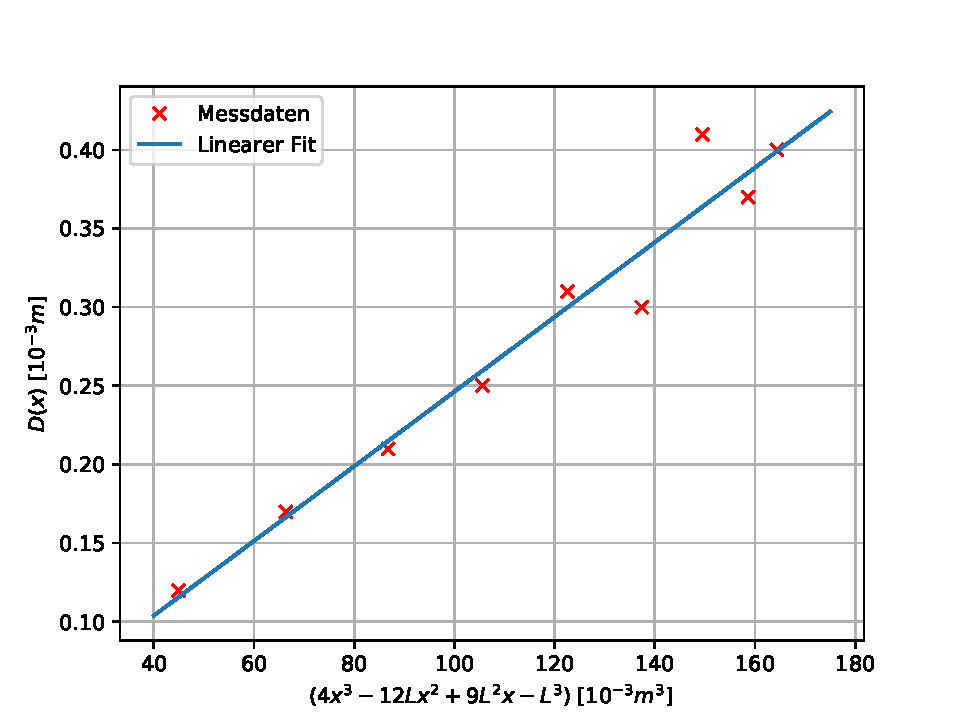
\includegraphics{content/plots/rundb2.pdf}
  \caption{Lineare Regression: runder Stab, beidseitige Auflage, $X>L/2$}
  \label{fig:LinRegrundb2}
\end{figure}

rundb2:
a = 0.002373265473474495 ± 0.000196410962171616
b = 0.009000034335808427 ± 0.02392505292907706

\pagebreak

\subsection{eckiger Stab, einseitige Einspannung}

\begin{table}
  \centering
  \caption{Messung der Biegung des eckigen Stabs bei einseitiger Einspannung}
  \label{tab:ecks}
  \sisetup{table-format=2.1}
  \begin{tabular}{S[table-format=3.0] S[table-format=1.2]}
    \toprule
    {$x \mathbin{/} \si{\milli\meter}$} & {$D(x) \mathbin{/} \si{\milli\meter}$}\\
    \midrule
    100 & 0,32\\
    125 & 0,46\\
    150 & 0,62\\
    175 & 0,73\\
    200 & 0,87\\
    225 & 1,03\\
    250 & 1,15\\
    275 & 1,32\\
    300 & 1,64\\
    325 & 1,86\\
    350 & 2,01\\
    375 & 2,32\\
    400 & 2,68\\
    425 & 2,90\\
    450 & 3,05\\
    475 & 3,44\\
    500 & 3,75\\
    525 & 4,11\\
    \bottomrule
  \end{tabular}
\end{table}



\pagebreak

\subsection{eckiger Stab, beidseitige Auflage}
\begin{table}
  \centering
  \caption{Messung der Biegung des eckigen Stabs bei beidseitiger Auflage}
  \label{tab:eckb}
  \sisetup{table-format=2.1}
  \begin{tabular}{S[table-format=3.0] S[table-format=1.2]}
    \toprule
    {$x \mathbin{/} \si{\milli\meter}$} & {$D(x) \mathbin{/} \si{\milli\meter}$}\\
    \midrule
    50 & 0,01\\
    75 & 0,03\\
    100 & 0,06\\
    125 & 0,07\\
    150 & 0,08\\
    175 & 0,11\\
    200 & 0,14\\
    225 & 0,15\\
    250 & 0,16\\
    275 \\
    300 & 0,18\\
    325 & 0,17\\
    350 & 0,16\\
    375 & 0,15\\
    400 & 0,12\\
    425 & 0,12\\
    450 & 0,10\\
    475 & 0,08\\
    500 & 0,04\\
    \bottomrule
  \end{tabular}
\end{table}



